%Vorlesung vom 14.12.17
\section{Fortsetzung lineare Regressionsmodelle}
\textbf{1.Frage}: Ob es einen Zusammenhang zwischen $X_i$ und $Y$ gibt? \\
\textbf{2.Frage}: Welche Kovariablen haben einen Effekt auf $Y$? \\
\textbf{3.Frage}: Wie gut repräsentiert das multivariate Regressionsmodell die beobachtete Varianz von $Y$?\\

\subsection{Gibt es einen Zusammenhang} F-Test\\
Beantwortet: Hat mindestens eine der Kovariablen einen Effekt.
\[ H_0: \beta_1=\beta_2=\dots=\beta_p=0 \]
\[ H_1: \beta_j \neq 0 \]
\[F= \frac{\text{erklärte Varianz}}{\text{unerklärte Varianz}} = \frac{\frac{TSS - RSS}{p}}{\frac{RSS}{n-p-1}} \]
\begin{itemize}
	\item $H_0$ kann nicht abgelehnt werden, wenn $F \sim 1$
	\item $H_1$ kann abgelehnt werden, wenn $F > 1$
\end{itemize}

\subsection{Welche der Kovariablen haben einen Effekt}
Jede einzelne Koeffizient $\beta_1,\dots,\beta_p$ kann mittels einen t-Tests getestet werden:
\[ H_0: \beta_j = 0 \]
\[H_1: \beta_j \neq 0 \]
\[ t= \frac{\hat{\beta_j}}{sd(\beta_j)} \]
adjustierte p-Werte: \\
$\Rightarrow$ Bonferroni-Korrektur
$\Rightarrow$ Benjamin-Hochberg

\subsection{Güte des Fits}
\[ R^{2} = \frac{\text{erklärte Varianz}}{\text{unerklärte Varianz}} = \frac{TSS -RSS}{TSS} \]
\[ \text{adjustiertes} R_{adj}^{2} = 1 - \frac{\frac{TSS - RSS}{p}}{\frac{RSS}{n-p-1}} \]

\section{Qualitative Kovariablen}
In Genexpressionsanalysen ist man oft daran interessiert, den Effekt von kategorialen Variablen zu untersuchen.\\
$\Rightarrow$ Kategoriale und quantitative Variablen können im selben Modell aufgenommen werden \\
$\Rightarrow$ Kategoriale Variablen werden mittels sog. Dummy-Variablen kodiert:
	\begin{itemize}
		\item \#Kategorien = 2 $\Rightarrow$ als binäre Variable kodiert
		\item \#Kategorien $>$ 2 $\Rightarrow$ meherere binäre Variablen
	\end{itemize}

\subsection{Treatment-Contrast Parametrisierung}
\[ X_i = \begin{cases}
		1, i \hat{=} \text{ level 1 (female)} \\
		0, i \hat{=} \text{ level 2 (male)}
\end{cases} \]

\[ Y = \begin{cases}
		\beta_0 + \beta_1 + \epsilon, \text{ falls } i = \text{ level 1 } \\
		\beta_0 + \epsilon, \text{ falls } i = \text{ level 2 } \\
\end{cases} \]

$\beta_0:$ Mittlerer Effekt von level 2\\
$\beta_1:$ Mittlere Differenz zwischen level 1 und level 2\\

\subsection{Group-Means-Parametrisierung}
\[ X_i = \begin{cases}
		1, i \hat{=} \text{ level 1 (female)} \\
		-1, i \hat{=} \text{ level 2 (male)}
\end{cases} \]

\[ Y = \begin{cases}
		\beta_0 + \beta_1 + \epsilon, \text{ falls } i = \text{ level 1 } \\
		\beta_0 - \beta_1 + \epsilon, \text{ falls } i = \text{ level 2 } \\
\end{cases} \]
$\beta_0:$ Mittlerer Effekt (unabhängig vom gewählten Level)\\
$\beta_1:$ Anteil den Level 1 größer als der mitlere Effekt ist bzw. den Anteil von Level 2, der kleiner als der mittlere Effekt ist\\

\section{Annahmen für lineare Regressionsmodelle}
\begin{enumerate}
	\item Zusammenhang ist (annähernd linear)
	\item Kovariablen sind unabhängig (keine Kolinearität)
	\item Fehlreterme eine konstante Varianz haben $\epsilon_i \sim N(0, \sigma^{2} )$ (Homoskedastizität)
\end{enumerate}
$\Rightarrow$ Diagnostik für lineare Modelle

\subsection{Test auf Annahme 1}
$\Rightarrow$ Residualplot
$\Rightarrow$ Dieser sollte keine Muster in der Punktwolke erkennen lassen. Denn bei linearem Zusammenhang sollten die Residuen zufällig um vorhergesagten Werte $\hat{y_i}$ streuen

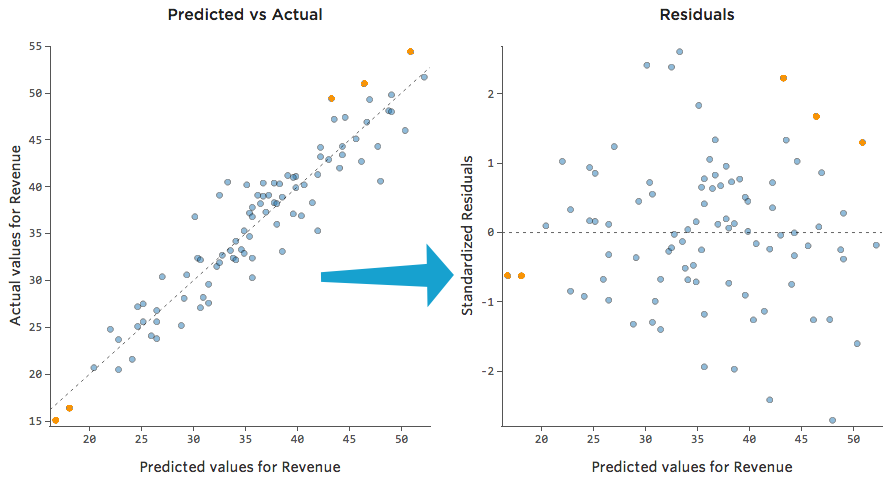
\includegraphics[scale=0.4]{VorlesungenTexDateien/images/residual}
\todo{Kein Muster erkennbar}
       
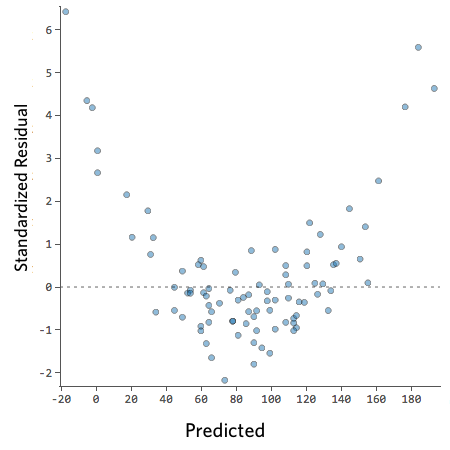
\includegraphics[scale=0.5]{VorlesungenTexDateien/images/Nonlinear-residual-11}
\todo{Nonlinearer Zusammenhang erkennbar}

\subsection{Test auf Annahme 2}
Kollinearität wird beobachtet, falls 2 oder meherere Variablen linear abhängig voneinander sind.

\[ X_i = \lambda_0 + \lambda_1 X_i \]

Variance Inflation Faktor (VIF):
\[ VIF(\hat{\beta_j})= \frac{1}{1- R_{X_j|X_{p \neq j}}^{2}} \]
\[ R_{X_j|X_{p \neq j}}^{2} \sim 1 \Rightarrow VIF >> 1 \]

\paragraph{Probleme bei Kollinearität}
\begin{enumerate}
	\item Es ist nicht möglich den Effekt den die abhängigen Kovariablen auf  haben voneinander zu trennen
	\item $sd(\hat{\beta_i})$ ist erhöht, denn: 
		\begin{itemize}
			\item Annahme für $\beta_i$: gibt den Effekt von $X_i$ auf $Y$ an $\Leftrightarrow$ alle anderen Kovariablen konstant sind
			\item Falls aber $X_i$ und $X_j$ linear abhängig sind, dann gibt es viele Wertepaare von $\beta_i$ und $\beta_j$, die nun einen ähnlichen Fehler (RSS) haben
		\end{itemize}
		$\Rightarrow$ Schätzer $\hat{\beta_i}$ und $\hat{\beta_j}$ sind ungenauer \\
		$\Rightarrow$ geringere Power für t-Test
\end{enumerate}

\paragraph{Wie kann mit Kollinearität umgegangen werden?}
\begin{enumerate}
	\item Entferne alle bis auf eine der linear abhängigen Kovariablen
	\item Fasse linear abhängige Kovariablen in einer neuen Kovariablen zusammen z.B. durch Bildung des Mittelwertes \\
		Beachte: Es kann notwendig sein, diese Kovariablen vorher zu standardisieren
\end{enumerate}

\subsection{Test auf Annahme 3}
Homoskedastizität ist gegeben, falls Fehlerterme $\epsilon_i$ eine konstante Varianz
\[ Var(\epsilon_i) = \sigma_{\epsilon}^{2} \text{ für alle  Beobachtungen } (x_i, y_i) \] 
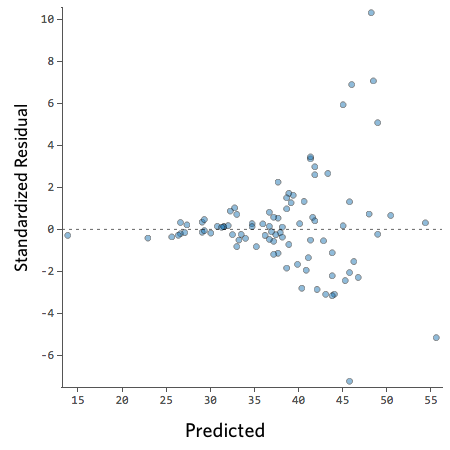
\includegraphics[scale=0.5]{VorlesungenTexDateien/images/Heteroscadicity}
\todo{Trichterform $\Rightarrow$ Heteroskedastizität}

\paragraph{Wie wird mit Heteroskedastizität umgegangen}
\begin{enumerate}
	\item Stabilisieren die Varianz der Fehler:\\
		Werte für $Y$ so transformiert werden, dass größere Werte kleinere Werte annehmen:
		\begin{enumerate}
			\item $log(Y)$
			\item $glog(Y) = log_{2}(\frac{1}{2} y + \frac{1}{2}\sqrt{y^{2} + a^{2}} ) $ \\
				$\Rightarrow$ Interpoliert $y$-Werte zwischen $log_2(Y)$ für große Werte von $Y$ und für kleine $\frac{y}{a} + log_2(\frac{a}{2})$
		\end{enumerate}
\end{enumerate}
